\documentclass[a4paper]{scrartcl}
\usepackage[utf8]{inputenc}
\usepackage[english]{babel}
\usepackage{graphicx}
\usepackage{lastpage}
\usepackage{pgf}
\usepackage{wrapfig}
\usepackage{fancyvrb}
\usepackage{fancyhdr}
\usepackage{hyperref}
\pagestyle{fancy}

\catcode`\_=\active
\protected\def_#1_{\textit{#1}}

% Create header and footer
\headheight 27pt
\pagestyle{fancyplain}
\lhead{\footnotesize{Network Programming, ID1212}}
\chead{\footnotesize{RMI \& DBA}}
\rhead{}
\lfoot{}
\cfoot{\thepage}
\rfoot{}

% Create title page
\title{Assignment 3 - RMI \& DBA}
\subtitle{Network Programming, ID1212}
\author{Bernardo Gonzalez Riede, begr@kth.se}
\date{\today}

\begin{document}

\maketitle


\section{Introduction}

High level goals for this assignment.
\begin{itemize}
    \item Development of application which uses remote method invocation, RMI.
    \item Development of application which stores persistent data on a database.
\end{itemize}


\section{Literature Study}

Only the videos were used as re-introduction to JDBC and RMI since I have used JDBC and RMI in the past, although that was a few years ago.
Important for RMI is the creation of Interfaces to which caller has access.
The callee will have an implementation of it which gets called instead of the interface.
Because its a subclass, it can be used everywhere where the subclass (the interface) is expected.


In regards to the persistent storage, prepared statements are best practice and should always be used.

\section{Method}
As in previous assignments, the mvc approach has been used again to layer the program.

The choice for a database fell on MySQL because of past works with it.
The implementation was realized in Netbeans in Java 8 EE.


\section{Result}

Link to public Github repository with code:
\href{https://github.com/MemBernd/ID1212-RMI-DBA}{https://github.com/MemBernd/ID1212-RMI-DBA}

\subsection{Layering}

The client is divided as follows:
\begin{itemize}
    \item A startup layer for starting the client side.
    \item A view layer consisting of the, now familiar, classes similar to previous assignments.
\end{itemize}

The server consist of several layers.
\begin{itemize}
    \item The _server.controller.Controller_ acts as the view of the server side, initiating the events when called by the client through RMI.
        The _controller_ accesses the _model_ layer for functionality of retrieving the reference to the client, it's username etc.
    \item _ClientHandler_ in the _model_ layer has access to the storage layer to retrieve the data.
    \item _DBStorage_ in the _storage_ layer is the only class with actual knowledge about the implementation of persistent storage, in this case MySQL.
    \item The server gets started by a dedicated server.startup.ServerStartup.
\end{itemize}

A additional package _common_ holds the interfaces needed for RMI, a _FileHolder_ class and a custom Exception.


%subsection covering persistent storage stuff
\subsection{DBA}
The persistent storage solution was implemented using MySQL.
Every file has the following metadata:
\begin{itemize}
    \item A unique filename.
    \item Size (in bytes).
    \item name of the owner.
    \item Permissions whether its a private or public file and if read or write is allowed for public access.
\end{itemize}

In conjunction with storing username and password for a given user, the resulting database schema is as shown in \ref{fig:database}.

\begin{figure}[h!]
  \begin{center}
    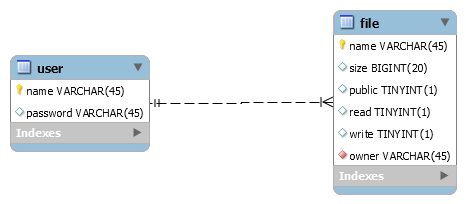
\includegraphics[scale=0.8]{db.png}
    \caption{Table relations in database.}
    \label{fig:database}
  \end{center}
\end{figure}

To increase performance, prepared statements have been used which get initialized at the creation of the server.storage.DBStorage (l. 148+).


%subsection covering rmi stuff
\subsection{RMI}

RMI is covered by registering an implementation of the common.Server interface in server.startup.ServerStartup, line 23.
This interface and therefore its implementations include the following functions:
\begin{itemize}
    \item _register()_ to register a new user.
    \item _unregister()_ to delete an existent user.
    \item _login()_ for login a user in.
    \item _logout()_ to logout.
    \item _list()_ to list all the files the user is allowed to see.
    \item _upload()_ to upload a new or a changed file.
    \item _download()_ to download a file.
    \item _delete()_ for deleting an existing file on the server.
    \item _addNotification()_ to add a listener to changes in a file.
\end{itemize}

As for the Client, he implements common.Client which only holds functions to print something out on his command line.
Its implementation client.View.Interpreter.ConsoleOutput, is passed when the user tries to login to the system and stored for future reference.

%subsection about permission management
\subsection{Permission management}
When a user tries to login, the username and password are matched to the database in DBStorage (l. 95+).
The controller uses the returned boolean (through the model) to either generate an random id (l. 54) to be returned to the client or to raise an AccessException.


This id is used as a token for the user to identify himself during the session.
All other method calls to the server which require authentication require this token to be passed along.

ClientHandler (the model) holds three Hashmaps (l. 24 - 26):
\begin{itemize}
    \item _clients_ to be able to retrieve the rmi reference received when logging in.
    \item _clientNames_ to be able to retrieve the username for owner matching of a file.
    \item _clientsToNotify_ for knowing if there's someone who needs to be notified about a change.
\end{itemize}
The first two use the id generated as a key, while the last one uses  the file's name.
Because the file name is unique and only the owner can request to be notified it was done this way.


Additionally, the ClientHandler includes two methods (l. 85 - 105) to be able to check if the user is allowed to read or write a given file.
If the user is not allowed to realize the operation, a _AccessException_ is raised with a message explaining what failed.

\subsection{Notification}

An assumption has been made; only the owner of a file can request to be notified about changes in his public files.
If he's the owner, an entry in the _clientsToNotify_ is made. This list is checked at every successful execution of uploading, downloading or deleting a file, e.g. server.controller.Controller (l. 89).

\subsection{UI}
Simplistic command line interface in \ref{fig:ui}.

\begin{figure}[h!]
  \begin{center}
    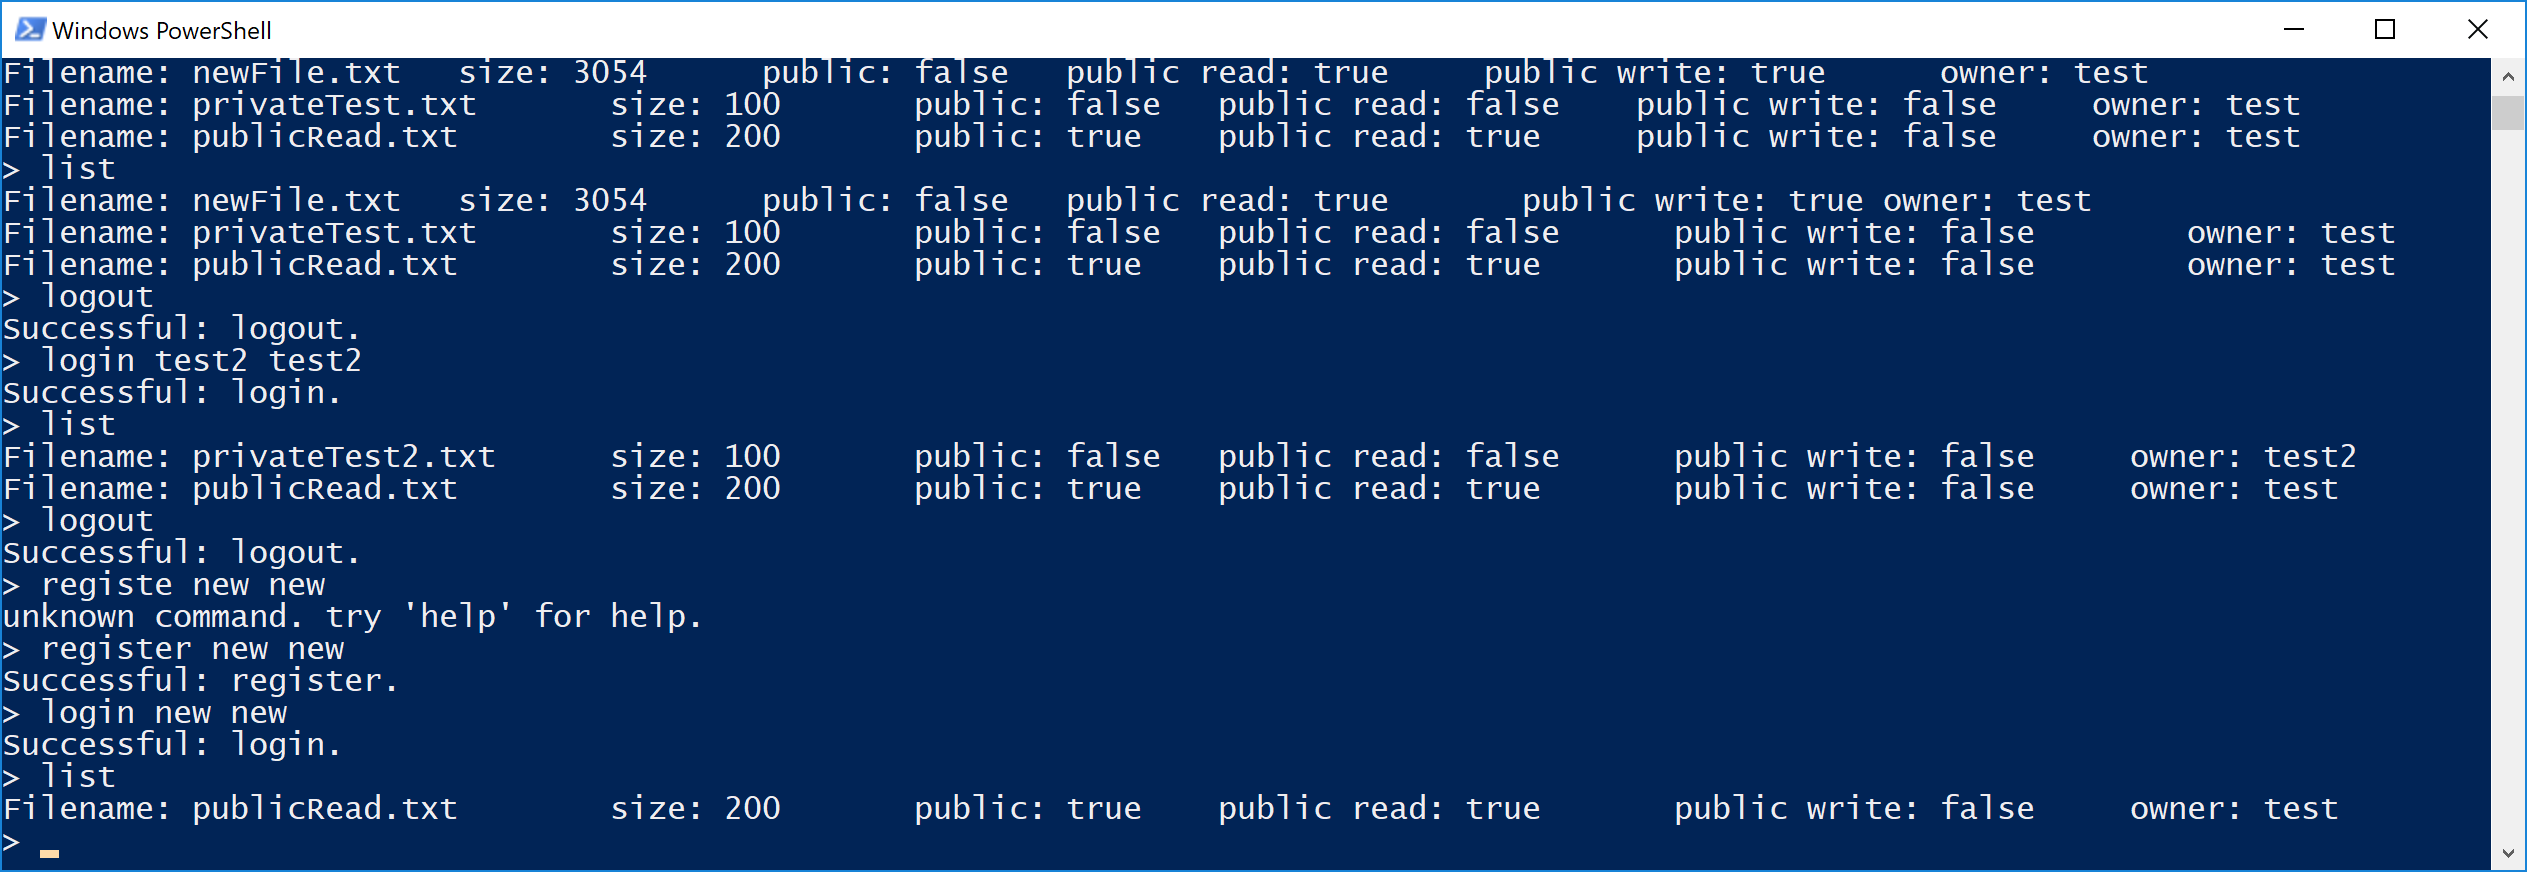
\includegraphics[scale=0.5]{ui.png}
    \caption{Several user listing files.}
    \label{fig:ui}
  \end{center}
\end{figure}

\section{Discussion}
The server.controller.Controller needs to be cleaned. it executes the same sequence at the beginning of most of the methods to validate the user.

Moreover, I'm not sure about best practices regarding the handling of output  from a method call to the server. I've used mostly exception which get caught by the client, but is this the ideal way to do it? 
Or is it better to use the reference provided by the client to write output to its command line? 
I'd appreciate a comment on this.

\section{Comments About the Course}

The time invested in this project were almost 12 hours.
\begin{itemize}
        \item 7h 35 min for coding.
        \item 1h 50 min for the report.
        \item 2h 40 min watching videos, taking notes and thinking about how to tackle the problem.
\end{itemize}

Albeit being intimidated about the task at the beginning, because of the discussion about the length of the program, I'm surprised to find out that the time needed was actually lower than in previous assignment.
Of course this is in regard to the work submitted, so the outcome will determine if it was indeed easier.


Disclaimer: I have been shown RMI and DBA to MySQL around 3 years before, resulting in an almost immediate understanding of the example code.


\end{document}
